% --- sections/3_methodology.tex ---

% --- Section 3.0: Methodology ---
% [METHODOLOGY AND PROJECT DESIGN] ensures it appears uppercase in the Table of Contents
\section[METHODOLOGY AND PROJECT DESIGN]{Methodology and Project Design}

\paragraph{ Rationale for Chosen Methods: }

\begin{itemize}
    \item \textbf{Multimodal Fusion:} Single-modality systems (keystroke only) are prone to mimicry attacks. Fusion with mouse dynamics increases the entropy of the user profile, making forgery exponentially harder \cite{mondal2017continuous}.
    
    

    \item \textbf{Deep \ac{SVDD} \& \acp{LSTM}:} Unlike static classifiers (e.g., \ac{SVM}), \ac{LSTM} networks are selected for their ability to model the temporal dependencies in sequential data \cite{kiyani2020continuous}. \ac{Deep SVDD} is chosen as the anomaly detector because it is a "one-class" classifier, meaning it can train on only the legitimate user's data without requiring impostor data during the training phase \cite{ruff2018deepsvdd, kim2024kdprint}.
    
    

    \item \textbf{\ac{JL} Lemma: } To counter the computational overhead of \ac{HE} \cite{cheon2017homomorphic}, the \ac{JL} Lemma \cite{johnson1984extensions} is applied to project high-dimensional biometric feature vectors into a lower-dimensional space. This allows for faster encrypted computations with mathematically guaranteed distance preservation \cite{rahman2021scalable}.

\end{itemize}
% This section outlines how you will conduct your research.
% It should be detailed enough that another researcher could replicate your study.

\subsection{Overview of the Proposed Methodology/Research Design}

\begin{enumerate}
    \item  \textbf{Feature Extraction \& Temporal Fusion:} The system ingests raw event logs and converts them into synchronized time-series feature vectors.
    
    \begin{itemize}
        \item \textbf{Keystroke Features:} Extraction of Flight Time (latency between KeyUP$_{n}$ $\rightarrow$ KeyDOWN$_{n+1}$) and \textit{Dwell Time} (duration of KeyDOWN$_{n}$ $\rightarrow$ KeyUP$_{n}$) \cite{gaines1980authentication, joyce1990identity}.
        
        
        
        \item \textbf{Mouse Features:} Calculation of higher-order motor metrics including Velocity Profiles, Angular Velocity, and Curvature Distance Ratio (efficiency of movement) \cite{ahmed2007new, zheng2011efficient}.
        
        
        
        \item \textbf{Multimodal Fusion:} The two independent streams are aligned using sliding time windows (e.g., $t=10s$) to create unified "behavioral frames" representing the user's complete interaction state \cite{mondal2017continuous, kiyani2020continuous}.
    \end{itemize}

    \begin{table}[H]
    \centering
    \caption{Technical Specification of Extracted Behavioral Features}
    \label{tab:feature_engineering}
    \begin{tabularx}{\textwidth}{@{}l l X X@{}}
        \toprule
        \textbf{Category} & \textbf{Modality} & \textbf{Specific Metrics} & \textbf{Rationale} \\ \midrule
        \textbf{Temporal} & Keystroke & Dwell Time, Flight Time \cite{gaines1980authentication, joyce1990identity, kiyani2020continuous} & Captures unique typing rhythm and biomechanical speed \cite{pirzado2021keystroke, shepherd1995continuous}. \\ \addlinespace
        \textbf{Kinematic} & Mouse & Velocity Profiles, Angular Velocity \cite{ahmed2007new, zheng2011efficient} & Distinguishes fine-grained motor-skill characteristics \cite{ahmed2007new}. \\ \addlinespace
        \textbf{Trajectory} & Mouse & Curvature Distance Ratio, Movement Efficiency \cite{mondal2017continuous, zheng2011efficient} & Measures hand stability and trajectory optimization \cite{mondal2017continuous}. \\ \addlinespace
        \textbf{Sequential} & Multimodal & Sliding Window Vectors (e.g., $t=10s$) \cite{kiyani2020continuous} & Synchronizes independent streams for continuous monitoring \cite{mondal2017continuous}. \\ \bottomrule
    \end{tabularx}
\end{table}
    

\item \textbf{Dimensionality Reduction (JL Layer):} To mitigate the "curse of dimensionality" caused by fusing two biometric streams, the high-dimensional fused vector ($d$) is projected onto a lower-dimensional subspace ($k$, where $k \ll d$) using the \ac{JL} Lemma \cite{johnson1984extensions}. This is achieved by multiplying the feature vector by a sparse random matrix ($R$) to produce a compressed, privacy-hardened embedding.
    
    
    
    \item \textbf{Privacy-Preserving Transformation:} The compressed embeddings are encrypted using a \textbf{\ac{LHE}} scheme (e.g., \ac{CKKS}) \cite{cheon2017homomorphic}. Unlike additive-only schemes, \ac{CKKS} supports the approximate arithmetic and multiplication depth required to compute \textit{squared Euclidean distances} ($||x - c||^2$) directly on the ciphertext. This ensures that the mathematical operations needed for authentication are performed entirely in the encrypted domain without decrypting the user's behavioral template \cite{rahman2021scalable}.
    
    

\item \textbf{Anomaly Detection (Deep SVDD):} The encrypted feature vectors are fed into a \ac{Deep SVDD} model \cite{ruff2018deepsvdd}. This model learns a compact hypersphere boundary encapsulating the legitimate user's ``normal'' behavior. During the verification phase, the system calculates the distance between the encrypted input and the hypersphere center; any input falling outside this learned radius is flagged as an anomaly (potential impostor) while the data remains mathematically indistinguishable from random noise under \ac{IND-CPA} security \cite{kim2024kdprint, ruff2018deepsvdd}.


\end{enumerate}

\begin{figure}[H]
    \centering
    \begin{tikzpicture}[scale=1.2]
        % --- Define Styles ---
        \tikzstyle{genuine}=[circle, fill=blue!70, inner sep=1.5pt]
        \tikzstyle{imposter}=[regular polygon, regular polygon sides=3, fill=red!70, inner sep=1.2pt, rotate=0]

        % --- The Hypersphere (Decision Boundary) ---
        \draw[thick, blue!80!black, fill=blue!5] (0,0) circle (2.5cm);
        \node[blue!80!black] at (0, 2.7) {\textbf{Learned Boundary (Hypersphere)}};

        % --- Center Point ---
        \fill[black] (0,0) circle (2pt) node[below right] {Center $c$};

        % --- Radius Arrow ---
        \draw[->, thick, black] (0,0) -- (1.76, 1.76) node[midway, above, sloped] {Radius $R$};

        % --- Genuine User Data (Inside) ---
        % Randomly distributed blue dots near the center
        \foreach \x/\y in {
            0.2/0.5, -0.3/0.8, 0.8/-0.2, -0.5/-0.5, 1.2/0.3,
            -1.0/0.4, 0.1/-1.2, 0.5/1.1, -0.8/-0.8, 1.5/-0.5,
            -0.2/1.5, 0.9/0.9, -1.2/-0.2, 0.4/-0.4, -0.1/0.1,
            0.6/-0.9, -0.6/0.6, 1.1/1.1, -1.4/0.5, 0.0/-1.5
        } {
            \node[genuine] at (\x, \y) {};
        }
        % Label for Genuine
        \node[blue!80!black, align=center] at (0, -0.5) {\small Genuine User\\ \small (Normal)};

        % --- Imposter Data (Outside) ---
        % Randomly distributed red triangles outside the circle
        \foreach \x/\y in {
            3.0/0.5, -3.2/1.2, 2.8/-2.0, -2.5/-2.5, 0.0/3.2,
            -3.5/0.0, 3.2/-0.5, 1.5/3.0, -1.0/-3.2, 2.2/2.2,
            -2.8/1.5, 3.1/-1.5, -2.0/2.8, 1.0/-3.0, -0.5/3.5
        } {
            \node[imposter] at (\x, \y) {};
        }
        % Label for Imposter
        \node[red!80!black, align=center] at (3.5, 0) {\small Imposter\\ \small (Anomaly)};
        \draw[->, red, thin] (3.0, 0.2) -- (2.6, 0.1); % Small pointer

        % --- Explanatory Labels ---
        \node[align=center, anchor=north] at (0, -2.8) {
            \textit{Objective:} Minimize $R^2 + \frac{1}{\nu} \sum \xi_i$ \\
            \footnotesize (Enclose genuine points, reject anomalies)
        };

    \end{tikzpicture}
    \caption{Visualizing the Deep SVDD Decision Boundary. The model learns a compact hypersphere of radius $R$ around center $c$ that encapsulates the majority of legitimate user data (blue dots). Any input falling outside this boundary is flagged as an anomaly (red triangles), representing a potential impostor.}
    \label{fig:deep_svdd_concept}
\end{figure}


\subsubsection{Architectural Design Mode I: Cryptographic Privacy (High-Security)}
\textit{Illustrated in Figure 1.} This mode is designed for high-risk transaction scenarios, such as banking login or authorizing payments. It utilizes \textbf{\ac{LHE} (\ac{CKKS})} \cite{cheon2017homomorphic} to perform anomaly detection inference entirely within the encrypted domain.



\begin{itemize}
    \item \textbf{Privacy Mechanism:} The behavioral template is encrypted using standard cryptographic protocols, ensuring mathematically provable security (\ac{IND-CPA}) \cite{cheon2017homomorphic}.
    \item \textbf{Trade-off:} While this offers the highest level of data protection, it incurs a higher computational cost, making it suitable for periodic, critical authentication rather than continuous, sub-second monitoring \cite{rahman2021scalable}.
\end{itemize}


\begin{figure}[H]
    \centering
    % Resize the diagram to fit the text width automatically
    \resizebox{\textwidth}{!}{%
    \begin{tikzpicture}[
        auto,
        node distance = 1.0cm and 1.0cm, % Reduced spacing between nodes
        % Define styles for the blocks
        input/.style = {rectangle, draw, fill=blue!10, text centered, rounded corners, minimum height=0.8cm, minimum width=2.2cm, font=\small},
        process/.style = {rectangle, draw, fill=orange!10, text centered, minimum height=2cm, minimum width=2.8cm, align=center, font=\small},
        secure/.style = {rectangle, draw, fill=red!5, text centered, rounded corners, minimum height=2.2cm, minimum width=3.5cm, dashed, align=center, font=\small},
        decision/.style = {diamond, draw, fill=green!10, text centered, aspect=2, minimum width=2cm, minimum height=1cm, font=\small},
        output/.style = {ellipse, draw, fill=gray!20, text centered, minimum height=0.8cm, font=\small},
        line/.style = {draw, -{Latex[length=3mm]}, thick}
    ]

    % --- Nodes ---
    
    % Inputs (Stacked vertically)
    \node [input] (key) {Keystroke Logs};
    \node [input, below=0.5cm of key] (mouse) {Mouse Logs};

    % Step 1: Feature Extraction (Placed to the right of the center of inputs)
    \node [process, right=1.2cm of key, yshift=-0.5cm] (features) {\textbf{Feature Extraction} \\ \& Fusion \\ \footnotesize (Velocity, Flight Time)};
    
    % Step 2: JL Projection
    \node [process, right=1.2cm of features] (jl) {\textbf{JL Projection} \\ \footnotesize ($d \rightarrow k$ dims) \\ \footnotesize $R \times x$};

    % Step 3: Encryption & Model (Grouped for Privacy)
    \node [secure, right=1.2cm of jl] (model) {\textbf{Encrypted Inference} \\ \footnotesize Homomorphic Enc. (CKKS) \\ + \\ \footnotesize Deep SVDD ($||x-c||^2$)};

    % Step 4: Decision (Below the secure model)
    \node [decision, below=1.0cm of model] (decide) {Anomaly?};
    
    % Outputs
    \node [output, left=1cm of decide] (genuine) {\textbf{Genuine}};
    \node [output, right=1cm of decide] (imposter) {\textbf{Imposter}};

    % --- Paths ---
    
    % Input to Features
    \draw [line] (key) -| (features.160);
    \draw [line] (mouse) -| (features.200);

    % Features to JL
    \draw [line] (features) -- node[above, scale=0.7, align=center] {High-Dim ($d$)} (jl);

    % JL to Model
    \draw [line] (jl) -- node[above, scale=0.7, align=center] {Compressed ($k$)} (model);

    % Model to Decision
    \draw [line] (model) -- node[right, scale=0.7] {Score} (decide);

    % Decision Outcomes
    \draw [line] (decide) -- node[above, scale=0.7] {No} (genuine);
    \draw [line] (decide) -- node[above, scale=0.7] {Yes} (imposter);

    % --- Secure Box Label ---
    \node [above=0.1cm of model, text=red, font=\footnotesize\itshape] {Secure Execution Environment};

    \end{tikzpicture}
    } % End of resizebox
    \caption{System Architecture of the Proposed Lightweight Privacy-Preserving Framework.}
    \label{fig:sys_arch}
\end{figure}

\begin{itemize}
\item \textbf{Privacy Mechanism:} The behavioral template is encrypted using standard cryptographic protocols, ensuring mathematically provable security (\ac{IND-CPA}) \cite{cheon2017homomorphic}.
\item \textbf{Trade-off:} While this offers the highest level of data protection, it incurs a higher computational cost, making it suitable for periodic, critical authentication rather than continuous, sub-second monitoring \cite{rahman2021scalable}.
\end{itemize}





\subsubsection{Architectural Design Mode II: Projected Privacy (High-Performance)}
\textit{Illustrated in Figure 2.} This mode is designed for continuous, passive background monitoring. It removes the heavy encryption overhead and relies on the \textbf{Johnson-Lindenstrauss (JL) Projection} as a form of non-invertible compression.

\begin{figure}[H]
    \centering
    % Resize the diagram to fit the text width automatically
    \resizebox{\textwidth}{!}{%
    \begin{tikzpicture}[
        auto,
        node distance = 1.0cm and 1.5cm,
        % Define styles for the blocks
        input/.style = {rectangle, draw, fill=blue!10, text centered, rounded corners, minimum height=0.8cm, minimum width=2.5cm, font=\small},
        process/.style = {rectangle, draw, fill=orange!10, text centered, minimum height=2cm, minimum width=3.5cm, align=center, font=\small},
        secure/.style = {rectangle, draw, fill=green!10, text centered, rounded corners, minimum height=2cm, minimum width=3.5cm, dashed, align=center, font=\small},
        decision/.style = {diamond, draw, fill=gray!20, text centered, aspect=2, minimum width=2.5cm, minimum height=1cm, font=\small},
        output/.style = {ellipse, draw, fill=gray!10, text centered, minimum height=0.8cm, font=\small},
        line/.style = {draw, -{Latex[length=3mm]}, thick}
    ]

    % --- Nodes ---
    
    % Inputs
    \node [input] (key) {Keystroke Logs};
    \node [input, below=0.8cm of key] (mouse) {Mouse Logs};

    % Step 1: Feature Extraction
    \node [process, right=1.5cm of key, yshift=-0.5cm] (features) {\textbf{Feature Extraction} \\ \& Fusion \\ \footnotesize (Velocity, Flight Time)};
    
    % Step 2: JL Projection (Acting as Encryption)
    \node [secure, right=1.5cm of features] (jl) {\textbf{JL Projection} \\ \textit{(Privacy Layer)} \\ \footnotesize $d \rightarrow k$ dimensions \\ \footnotesize $R \times x$};

    % Step 3: Deep SVDD (Now running on projected data directly)
    \node [process, right=1.5cm of jl] (model) {\textbf{Deep SVDD} \\ \footnotesize Anomaly Detection \\ \footnotesize $||x_{proj} - c||^2$};

    % Step 4: Decision
    \node [decision, below=1.0cm of model] (decide) {Anomaly?};
    
    % Outputs
    \node [output, left=1cm of decide] (genuine) {\textbf{Genuine}};
    \node [output, right=1cm of decide] (imposter) {\textbf{Imposter}};

    % --- Paths ---
    
    % Input to Features
    \draw [line] (key) -| (features.160);
    \draw [line] (mouse) -| (features.200);

    % Features to JL
    \draw [line] (features) -- node[above, scale=0.7, align=center] {Raw Vector ($d$)} (jl);

    % JL to Model
    \draw [line] (jl) -- node[above, scale=0.7, align=center] {Projected ($k$)} (model);

    % Model to Decision
    \draw [line] (model) -- node[right, scale=0.7] {Score} (decide);

    % Decision Outcomes
    \draw [line] (decide) -- node[above, scale=0.7] {No} (genuine);
    \draw [line] (decide) -- node[above, scale=0.7] {Yes} (imposter);

    % --- Label for Privacy ---
    \node [above=0.1cm of jl, text=red!80!black, font=\footnotesize\itshape] {Irreversible Compression};

    \end{tikzpicture}
    }
    \caption{Proposed Lightweight Architecture: Using JL Projections as a Privacy-Preserving Transformation.}
    \label{fig:lightweight_arch}
\end{figure}

\begin{itemize}
    \item \textbf{Privacy Mechanism:} The JL projection acts as a ``computational privacy'' layer. By projecting data from a high-dimensional space ($d$) to a significantly lower-dimensional space ($k$, where $k \ll d$), the original features become mathematically indeterminate and resistant to reconstruction attacks.
    \item \textbf{Trade-off:} This mode achieves ultra-low latency ($<200$ms), enabling the system to authenticate the user continuously without draining battery life or causing input lag, while still maintaining a robust defense against feature recovery.
\end{itemize}


\begin{table}[htbp]
    \centering
    \caption{Feature Comparison of Architectural Modes}
    \label{tab:arch_comparison}
    \begin{tabularx}{\textwidth}{@{}lXX@{}}
        \toprule
        \textbf{Feature} & \textbf{Mode I: Cryptographic Privacy} & \textbf{Mode II: Projected Privacy} \\ \midrule
        Primary Goal & High-security (e.g., banking logins)  & Continuous passive monitoring \cite{suais2019bbmas} \\ \addlinespace
        Privacy Mechanism & \ac{LHE} (\ac{CKKS}) \cite{cheon2017homomorphic} & \ac{JL} Projection \cite{johnson1984extensions} \\ \addlinespace
        Security Guarantee & Mathematically provable (\ac{IND-CPA}) \cite{cheon2017homomorphic} & Computational privacy/Non-invertible \cite{ruff2018deepsvdd} \\ \addlinespace
        Latency Target & Higher (Suitable for periodic use) \cite{kiyani2020continuous} & Ultra-low ($< 200$ms)  \\ \addlinespace
        Computational Cost & High \cite{kiyani2020continuous} & Very Low  \\ \bottomrule
    \end{tabularx}
\end{table}



% Provide a high-level summary of your approach.
% You might want to include a system architecture diagram here later.
% Explain whether this is a quantitative, qualitative, or mixed-method study.

\subsection{Data Collection}

To ensure the proposed privacy-preserving framework is robust, scalable, and generalizes well to real-world scenarios, this research utilizes a \textbf{Hybrid Multi-Source Dataset} approach. Data is aggregated from five distinct, high-impact repositories, covering both fixed-text and free-text typing scenarios, as well as multimodal (Keystroke + Mouse) interactions.

\subsubsection{Primary Datasets (Multimodal \& Cross-Device)}
The core training and fusion phases utilize two datasets that offer high-granularity sensor data.

\begin{itemize}
    \item \textbf{\ac{SU-AIS} \ac{BB-MAS} \cite{suais2019bbmas}:} 
    This dataset serves as the primary source for training the \ac{SVDD} model due to its user volume and cross-device consistency.
    \begin{itemize}
        \item \textbf{Source:} \ac{SU-AIS}.
        \item \textbf{Population:} $N = 117$ unique subjects.
        \item \textbf{Volume:} Approximately 11,760 keystrokes per user (Desktop subset).
        \item \textbf{Relevance:} It allows for the analysis of behavioral stability across different physical interfaces.
    \end{itemize}

    \item \textbf{Edge Hill KMT \cite{edgehill2012dataset}:}
    This dataset is critical for the multimodal fusion layer, as it captures simultaneous mouse and keyboard interactions.
    \begin{itemize}
        \item \textbf{Source:} Edge Hill University, UK.
        \item \textbf{Scenario:} Financial form filling (names, addresses, credit card details), representing a high-security context.
        \item \textbf{Population:} 88 user sessions with 1,760 interaction instances.
        \item \textbf{Features:} Captures Keystroke, Mouse (trajectory, velocity, click), and Touchscreen events.
    \end{itemize}
\end{itemize}

\subsubsection{Benchmark Datasets (Scalability \& Standardization)}
To validate the model against state-of-the-art standards and ensure scalability, two benchmark datasets are employed.

\begin{itemize}
    \item \textbf{Aalto University ``136M Keystrokes'' Dataset \cite{dhakal2018136m}:}
    Used for transfer learning to pre-train the \ac{LSTM} feature extractors on general typing patterns.
    \begin{itemize}
        \item \textbf{Scale:} The largest available public keystroke dataset ($>136$ million keystrokes).
        \item \textbf{Population:} Over 168,000 participants.
        \item \textbf{Type:} Free-text typing collected via an online web test.
    \end{itemize}

    \item \textbf{\ac{CMU} Keystroke Dynamics Benchmark \cite{cmu2009benchmark}:}
    Used as a baseline control group to compare \acp{EER} against existing literature.
    \begin{itemize}
        \item \textbf{Source:} \ac{CMU} Biometrics Research.
        \item \textbf{Population:} 51 subjects.
        \item \textbf{Type:} Fixed-text password entry (e.g., string ``.tie5Roanl'').
    \end{itemize}
\end{itemize}

\subsubsection{Supplementary Data}
\begin{itemize}
    \item \textbf{Feature Engineered Mouse Data \cite{reddy2025mouse}:}
    A pre-processed dataset containing engineered features such as trajectory straightness, jitter, and movement efficiency. This is utilized to fine-tune the mouse dynamics anomaly detection module without requiring raw signal processing.
\end{itemize}

% Summary Table
\begin{table}[ht]
\centering
\caption{Summary of Experimental Datasets}
\label{tab:datasets}
\begin{tabularx}{\textwidth}{|l|l|c|X|}
\hline
\textbf{Dataset} & \textbf{Modality} & \textbf{Users} & \textbf{Primary Role} \\ \hline
Edge Hill KMT \cite{edgehill2012dataset} & Key + Mouse & 88 & Multimodal Fusion Training \\ \hline
\ac{SU-AIS} \ac{BB-MAS} \cite{suais2019bbmas} & Key + Sensors & 117 & \ac{DL} (\ac{LSTM}) Training \\ \hline
Aalto 136M \cite{dhakal2018136m} & Keystroke & 168k+ & Scalability \& Transfer Learning \\ \hline
\ac{CMU} Benchmark \cite{cmu2009benchmark} & Keystroke & 51 & Baseline Validation \\ \hline
Figshare Mouse \cite{reddy2025mouse} & Mouse & N/A & Feature Engineering \\ \hline
\end{tabularx}
\end{table}
% Describe your data sources.
% Are you using a public dataset (e.g., HMOG, UCI)? 
% Or are you collecting your own data? If so, describe the sensors and sampling rate.

\subsection{Ethical Considerations}

This research utilizes \textbf{secondary data} obtained from open-access academic repositories and public benchmarks (\ac{SU-AIS} \ac{BB-MAS} \cite{suais2019bbmas}, Edge Hill KMT \cite{edgehill2012dataset}, and Aalto University \cite{dhakal2018136m}). As such, this study does not involve direct interaction with human participants, and no new personal data collection is performed.

\paragraph{Data Privacy and Anonymity:}
The datasets used in this study have been previously de-identified by the original data custodians. All records are referenced by unique alphanumeric identifiers (e.g., \texttt{User\_001}), ensuring that no \textbf{\ac{PII}}---such as names, addresses, or actual passwords---is processed or accessible. 
\begin{itemize}
    \item In the \textbf{Edge Hill KMT dataset \cite{edgehill2012dataset}}, the original collection protocol ensured that users entered \textit{fictitious} financial information; thus, no real sensitive financial data is exposed.
    \item In the \textbf{\ac{SU-AIS} \ac{BB-MAS} dataset \cite{suais2019bbmas}}, demographic attributes (age, gender) are provided in an anonymized format that prevents the re-identification of specific individuals.
\end{itemize}

\paragraph{Compliance and Licensing:}
All data is used in strict accordance with their respective licensing agreements (e.g., Creative Commons Attribution 4.0 International). The data is utilized solely for the purpose of academic research to train and validate the proposed privacy-preserving authentication model. No attempt will be made to deanonymize the data subjects.

% Discuss any ethical issues related to your data or subjects.
% For behavioral biometrics, privacy is a key concern.
% Mention if you have or need IRB approval.

\subsection{Evaluation and Validation}

The performance of the proposed privacy-preserving authentication framework will be rigorously evaluated using a comprehensive suite of biometric and system performance metrics. The evaluation strategy is designed to quantify the trade-offs between authentication accuracy, computational latency, and privacy overhead.

\subsubsection{Experimental Design}
The validation process will follow a \textbf{$k$-fold Cross-Validation} ($k=10$) protocol to ensure statistical reliability. The dataset will be partitioned into:

\begin{figure}[H]
    \centering
    \resizebox{0.8\textwidth}{!}{%
    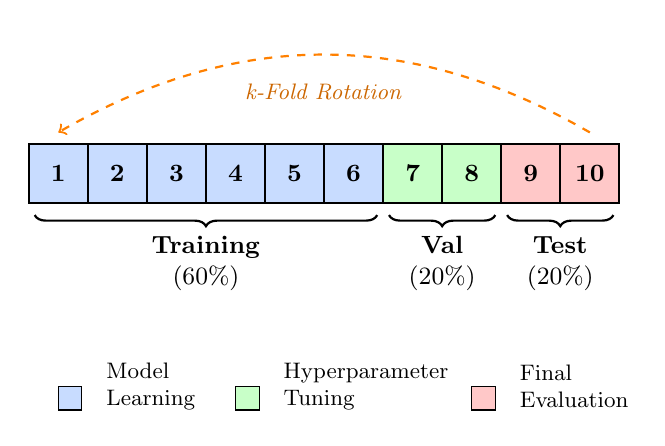
\begin{tikzpicture}[scale=0.75, font=\small]

    % --- Define Colors ---
    \definecolor{trainBlue}{RGB}{200, 220, 255}
    \definecolor{valGreen}{RGB}{200, 255, 200}
    \definecolor{testRed}{RGB}{255, 200, 200}

    % --- DRAW BLOCKS (Fold 1) ---
    \foreach \i in {1,...,10} {
        \ifnum \i < 7
            \def\col{trainBlue} 
        \else
            \ifnum \i < 9
                \def\col{valGreen}
            \else
                \def\col{testRed}
            \fi
        \fi
        \draw[fill=\col, thick] (\i-1, 0) rectangle (\i, 1);
        \node at (\i-0.5, 0.5) {\textbf{\i}};
    }

    % --- BRACE LABELS ---
    \draw[decorate, decoration={brace, amplitude=4pt, mirror}, thick] (0.1, -0.2) -- (5.9, -0.2) 
        node[midway, below=4pt, align=center] {\textbf{Training} \\ (60\%)};
    
    \draw[decorate, decoration={brace, amplitude=4pt, mirror}, thick] (6.1, -0.2) -- (7.9, -0.2) 
        node[midway, below=4pt, align=center] {\textbf{Val} \\ (20\%)};

    \draw[decorate, decoration={brace, amplitude=4pt, mirror}, thick] (8.1, -0.2) -- (9.9, -0.2) 
        node[midway, below=4pt, align=center] {\textbf{Test} \\ (20\%)};

    % --- ROTATION ARROW ---
    \draw[->, thick, dashed, orange] (9.5, 1.2) to[out=150, in=30] (0.5, 1.2);
    \node[above, text=orange!80!black, scale=0.9] at (5, 1.6) {\textit{k-Fold Rotation}};

    % --- LEGEND ---
    \begin{scope}[yshift=-3.5cm, xshift=0.5cm]
        \draw[fill=trainBlue] (0,0) rectangle (0.4,0.4) node[right=0.2cm, align=left, scale=0.9] {Model\\Learning};
        \draw[fill=valGreen] (3.0,0) rectangle (3.4,0.4) node[right=0.2cm, align=left, scale=0.9] {Hyperparameter\\Tuning};
        \draw[fill=testRed] (7.0,0) rectangle (7.4,0.4) node[right=0.2cm, align=left, scale=0.9] {Final\\Evaluation};
    \end{scope}

    \end{tikzpicture}
    }
    \caption{Experimental Data Partitioning Strategy. The dataset is divided into 10 folds with a 60/20/20 split for Training, Validation, and Testing. Assignments rotate cyclically.}
    \label{fig:k_fold_split}
\end{figure}

\begin{itemize}
    \item \textbf{Training Set (60\%):} Used to train the Deep \ac{SVDD} model \cite{ruff2018deepsvdd} to learn the user's normal behavioral boundary.
    \item \textbf{Validation Set (20\%):} Used for hyperparameter tuning (e.g., \ac{LSTM} layer size, \ac{JL} projection dimension $k$).
    \item \textbf{Testing Set (20\%):} Used to evaluate the final performance on unseen data.
\end{itemize}

To simulate real-world attacks, \textbf{Zero-Effort Impostor} testing will be conducted, where every other user in the dataset acts as an impostor against the target user.

\subsubsection{Biometric Performance Metrics}
The primary measure of authentication success is the system's ability to correctly distinguish the legitimate user from impostors.

\begin{itemize}
    \item \textbf{\ac{FAR}:} The probability that an unauthorized user (impostor) is incorrectly accepted by the system.
    \begin{equation}
        \eqname{False Acceptance Rate (FAR) Calculation}
        FAR = \frac{FP}{FP + TN} \times 100\%
        \label{eq:far}
    \end{equation}
    \textit{Where \ac{FP} is False Positives and \ac{TN} is True Negatives.}

    \item \textbf{\ac{FRR}:} The probability that the legitimate user is incorrectly rejected by the system.
    \begin{equation}
        \eqname{False Rejection Rate (FRR) Calculation}
        FRR = \frac{FN}{FN + TP} \times 100\%
        \label{eq:frr}
    \end{equation}
    \textit{Where \ac{FN} is False Negatives and \ac{TP} is True Positives.}

    \item \textbf{\ac{EER}:} The operating point where $FAR = FRR$. A lower \ac{EER} indicates a more accurate system.
    \begin{equation}
        \eqname{Equal Error Rate (EER) Equilibrium Point}
        EER = \{ FAR \mid FAR = FRR \}
        \label{eq:eer}
    \end{equation}
\end{itemize}



\subsubsection{System Efficiency \& Scalability Metrics}
To validate the effectiveness of the \textbf{\ac{JL} Lemma \cite{johnson1984extensions}} and \textbf{\ac{HE}}, the following computational metrics will be recorded:

\begin{itemize}
    \item \textbf{Inference Latency ($L_{inf}$):} The time taken to process a single authentication request.
    \begin{equation}
        \eqname{Total Pipeline Inference Latency}
        L_{inf} = T_{proj} + T_{enc} + T_{score}
        \label{eq:latency}
    \end{equation}
    \textit{Target:} $L_{inf} < 200$ms (Real-time threshold).

    \item \textbf{Encryption Overhead Ratio ($E_{ratio}$):} The ratio of processing time in the encrypted domain versus the plaintext domain.
    \begin{equation}
        \eqname{Homomorphic Encryption Computational Overhead Ratio}
        E_{ratio} = \frac{T_{encrypted}}{T_{plaintext}}
        \label{eq:overhead}
    \end{equation}
\end{itemize}

\subsubsection{Privacy and Security Evaluation}
Given the cybersecurity focus of this research, quantifying the strength of the privacy-preserving mechanisms is critical.

\begin{itemize}
    \item \textbf{Indistinguishability (Adversarial Advantage):} 
    To verify semantic security (\ac{IND-CPA} \cite{cheon2017homomorphic}), we measure the probability that an adversary $\mathcal{A}$ can distinguish between two encrypted biometric templates.
    \begin{equation}
        \eqname{Adversarial Advantage for IND-CPA Security Proof}
        Adv_{\mathcal{A}} = \left| \Pr[\mathcal{A}(E(m_0)) = 1] - \Pr[\mathcal{A}(E(m_1)) = 1] \right|
        \label{eq:adv_advantage}
    \end{equation}

    \item \textbf{Reconstruction Resistance (Feature Recovery Attack):}
    To simulate a database breach, an inverse-mapping \ac{DL} network (Decoder $\mathcal{D}$) will be trained to attempt to reconstruct the original raw features $X$ from the stored templates $T$. Privacy is quantified by the maximization of the Reconstruction Error (\ac{MSE}):
    \begin{equation}
        \eqname{Mean Squared Error for Template Reconstruction Resistance}
        MSE_{recon} = \frac{1}{N} \sum_{i=1}^{N} (X_i - \mathcal{D}(T_i))^2
        \label{eq:mse_recon}
    \end{equation}

    \item \textbf{Information Leakage (Mutual Information):}
    We quantify the dependency between the raw biometric vector $X$ and the projected/encrypted vector $Z$ using Shannon's Mutual Information:
    \begin{equation}
        \eqname{Shannon Mutual Information Leakage Between Raw and Encrypted Features}
        I(X; Z) = \sum_{x \in X} \sum_{z \in Z} p(x,z) \log \left( \frac{p(x,z)}{p(x)p(z)} \right)
        \label{eq:mutual_info}
    \end{equation}
\end{itemize}

% How will you measure success?
% metric examples:
